\documentclass[ebook,10pt,oneside,openany]{memoir}
\usepackage[utf8x]{inputenc}
\usepackage[english]{babel}
\usepackage{amsmath}
\usepackage{amssymb}
\usepackage{amsthm}
\usepackage{tikz}
\usetikzlibrary{calc}
\usepackage{collectbox}
\usepackage[normalem]{ulem}
\usepackage{mathrsfs}



\theoremstyle{plain}
\newtheorem{thm}{Theorem}[section]
\newtheorem{lem}[thm]{Lemma}
\newtheorem{prop}[thm]{Proposition}
\newtheorem*{cor}{Corollary}

\theoremstyle{definition}
\newtheorem{defn}{Definition}[section]
\newtheorem{ex}{Example}[section]
\newtheorem{conj}{Conjecture}[section]
\newtheorem{exmp}{Example}[section]

\theoremstyle{remark}
\newtheorem*{rem}{Remark}
\newtheorem*{note}{Note}
\newcommand{\N}{\mathbb{N}}
\newcommand{\Z}{\mathbb{Z}}
\newcommand{\Q}{\mathbb{Q}}
\newcommand{\R}{\mathbb{R}}
\newcommand{\K}{\mathbb{K}}
\newcommand{\C}{\mathbb{C}}
\newcommand{\ra}{\Rightarrow}
\newcommand{\la}{\leftarrow}

\newcommand{\mtwotwo}[4]{
\begin{bmatrix}
#1 & #2\\
#3 & #4
\end{bmatrix}
}

\newcommand{\mthreethree}[9]{
\begin{bmatrix}
#1 & #2 & #3\\
#4 & #5 & #6\\
#7 & #8 & #9
\end{bmatrix}
}

\newcommand{\mtwothree}[6]{
\begin{bmatrix}
#1 & #2 & #3\\
#4 & #5 & #6
\end{bmatrix}
}

\newcommand{\mthreetwo}[6]{
\begin{bmatrix}
#1 & #2\\
#3 & #4\\
#5 & #6
\end{bmatrix}
}





\title{MATH544 Notes}
\author{Justin Baum}

\begin{document}
\maketitle
\tableofcontents
\chapter{Pre-Class}
\section{Number Fields}
\begin{defn}
A field is any set $\K$ which follow the Field Axioms:
\begin{enumerate}
   \item $\alpha + \beta = \beta + \alpha$ (addition is commutative).
   \item $(\alpha + \beta) + \gamma =\alpha + (\beta + \gamma)$ (addition is associative).
   \item There exists an element $0$ such that $\alpha + 0 = \alpha$.
   \item For every $\alpha \in \K$, there exists $\beta$ such that $\alpha + \beta = 0$.
   \item $\alpha\beta = \beta\alpha$ (multiplication is commutative).
   \item $(\alpha\beta)\gamma = \alpha(\beta\gamma)$ (multiplication is associative).
   \item There exists an element $1$ such that $1\cdot \alpha = \alpha$.
   \item For every $\alpha$ there exists a $\gamma$ such that $\alpha\gamma = 1$.
   \item $\alpha(\beta + \gamma) = \alpha\beta + \alpha\gamma$, multiplication is distributive over addition.
\end{enumerate}
\end{defn}
\begin{defn}
Two fields, $\K$ and $\K'$ are said to be \textbf{isomorphic} if we can setup a one to one correspondence between $\K$ and $\K'$.
\end{defn}
The most common fields are, $\Q$, $\R$, $\C$.

\section{Theory of Linear Algebra}
Involving space, and the most general case, a series of linear equations.
\[a_{11}x_{11} + a_{12}x_{12} + \dots + a_{1n}x_{1n} = b_1\]
\[a_{21}x_{21} + a_{22}x_{22} + \dots + a_{2n}x_{2n} = b_2\]
\[\dots \dots \dots \dots \dots \dots \dots \dots \dots\]
\[a_{n1}x_{n1} + a_{n2}x_{n2} + \dots + a_{nn}x_{nn} = b_n\]

\section{Determinant}
The determinant is the scalar that a 1 area, volume, hypervolume etc. gets scaled by. Even a one length can be scaled or reduced to 0. When a determinant is 0, it means that all space, gets squished to a lower dimension and thus has 0 volume, or 0 area, and so on.
\[D = 
\begin{vmatrix}
a_{11} & a_{12} & \dots & a_{1n}\\
a_{21} & a_{22} & \dots & a_{2n}\\
\vdots & \vdots & \ddots & \vdots \\
a_{n1} & a_{2n} & \dots & a_{nn}
\end{vmatrix} = \det||a||
\]

\begin{figure}
  \centering
  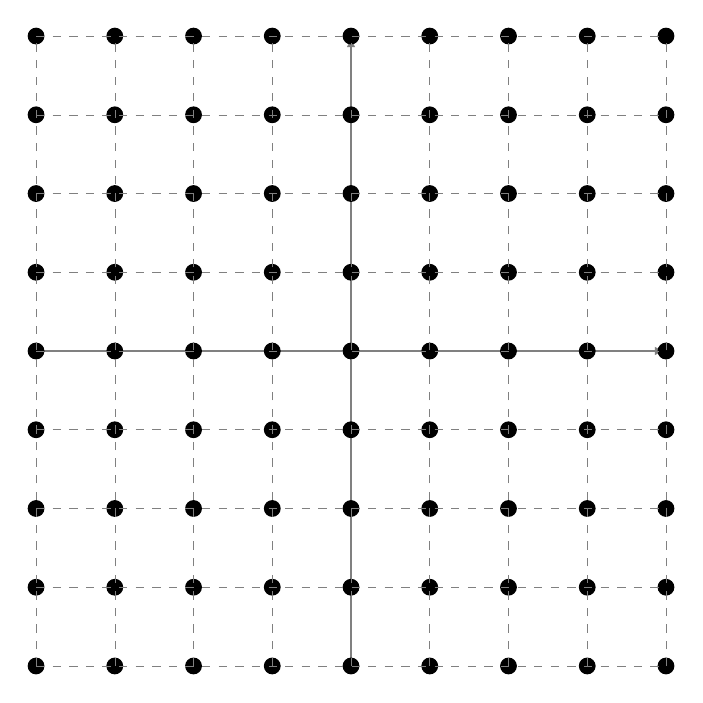
\begin{tikzpicture}[scale=1]
    \coordinate (Origin)   at (0,0);
    \coordinate (XAxisMin) at (-4,0);
    \coordinate (XAxisMax) at (4,0);
    \coordinate (YAxisMin) at (0,-4);
    \coordinate (YAxisMax) at (0, 4);
    \draw [thin, gray,-latex] (XAxisMin) -- (XAxisMax);% Draw x axis
    \draw [thin, gray,-latex] (YAxisMin) -- (YAxisMax);% Draw y axis

    %\clip (-3,-2) rectangle (10cm,10cm); % Clips the picture...
    \pgftransformcm{1}{0}{0}{1}{\pgfpoint{0cm}{0cm}}
          % This is actually the transformation matrix entries that
          % gives the slanted unit vectors. You might check it on
           % MATLAB etc. . I got it by guessing.
          % Draws a grid in the new coordinates.
    \foreach \x in {-4,-3,...,4}{% Two indices running over each
      \foreach \y in {-4,-3,...,4}{% node on the grid we have drawn 
        \node[draw,circle,inner sep=2pt,fill] at (\x,\y) {};
            % Places a dot at those points
      }
    }
    \draw[style=help lines,dashed] (-4,-4) grid[] (4,4);
  \end{tikzpicture}
  \caption{Vector Space $\R^2$ for $\forall (x,y); -4 \leq x \leq 4 and -4 \leq y \leq 4$.}
  \label{figure:solving-CVP-bad-basis}
\end{figure}

\section{Acknowledgements}
Almost none of this work is of my own. This work is from \textit{Linear Algebra} by George Shilov. And lecture notes from Dr. Matt Miller's MATH544H class taught at the University of South Carolina in the Spring of 2019.
\chapter{Lectures}
\section{14 January 2019}
\begin{defn}
Linear Algebra is the study of vector spaces and the maps between them.
\end{defn}

\begin{defn}
A function $T:V\to W$, from vector space $V$, the domain, to vector space $W$, the codomain, is called a linear transformation if
\[T(c\Vec{u}+\Vec{v})=cT(\Vec{u})+T(\Vec{v});\ \forall \Vec{u},\Vec{v}\in V \wedge c\in \R\]
\end{defn}

\begin{ex}
\[T:\R\to\R;\ T(x)=2x\]
\[T(cu+v) = 2cu + v = cT(u)+T(v)\]
So this is a linear transformation.
\end{ex}
\begin{ex}
\[C^0[0,2\pi] = \{f:[0,2\pi]\to\R\ |\ f\ is \ continuous\}\]
\[S:C^0[0,2\pi]\to \R\]
\[S(f) = f(\pi)\]
Check linearity.
\[S(cf+g) = (cf+g)(\pi)=cf(\pi)+g(\pi)=cS(f)+S(g)\]
\end{ex}

\begin{ex}
\[Let\ T:C^0[0,2\pi]\to \R\]
\[T(f)=\Bar{f}\]
\[T(f)=\frac{1}{2\pi}\int_0^{2\pi}f(x)\ dx\]
Check linearity.
\[T(cf+g)=\frac{1}{2\pi}\int_0^{2\pi}(cf+g)(x)\ dx\]
\[T(cf+g)=\frac{1}{2\pi}(c\int_0^{2\pi}f(x)\ dx+\int_0^{2\pi}g(x)\ dx)\]
\[T(cf+g)=cT(f)+T(g)\]
\end{ex}

$\R^2$ and $\R^3$ are vector spaces, $(x,y)$ is mapped to the vector $\begin{bmatrix}x\\y
\end{bmatrix}$ and $(x,y,z)$ is mapped to the vector $\begin{bmatrix}x\\y\\z
\end{bmatrix}$.
\begin{ex}
Let $T:\R^2\to\R^3$ be defined by \[T(\begin{bmatrix}x\\y\end{bmatrix})=\begin{bmatrix}x+3y\\-x+y\\2x+y\end{bmatrix}\]
Verify linearity.
\[T(c\begin{bmatrix}x\\y\end{bmatrix}+\begin{bmatrix}z\\w\end{bmatrix})=T(\begin{bmatrix}cx+z\\cy+w\end{bmatrix}=\begin{bmatrix}cx+z+3cu+3w\\-cx-z+cy+w\\2cx+2z+cy+w\end{bmatrix}\]
\[T(c\begin{bmatrix}x\\y\end{bmatrix}+\begin{bmatrix}z\\w\end{bmatrix})=\begin{bmatrix}cx+3cu\\-cx+cy\\2cx+cy\end{bmatrix}+\begin{bmatrix}z+3w\\-z+w\\2z+w\end{bmatrix}\]
\[T(c\begin{bmatrix}x\\y\end{bmatrix}+\begin{bmatrix}z\\w\end{bmatrix})=c\begin{bmatrix}x+3u\\-x+y\\2x+y\end{bmatrix}+\begin{bmatrix}z+3w\\-z+w\\2z+w\end{bmatrix}\]
\[T(c\begin{bmatrix}x\\y\end{bmatrix}+\begin{bmatrix}z\\w\end{bmatrix})=cT(\begin{bmatrix}x\\y\end{bmatrix})+T(\begin{bmatrix}z\\w\end{bmatrix})\]
This transformation is the same as the matrix transformation, $\begin{bmatrix}1 & 3\\ -1 & 1\\ -2 & 1\end{bmatrix}$.
\end{ex}

\begin{defn}
Let $T: V\to W$ be a linear transformation. The range or image of $T$ is the is the set range $\mathscr{R}(T)$.
\begin{center}
    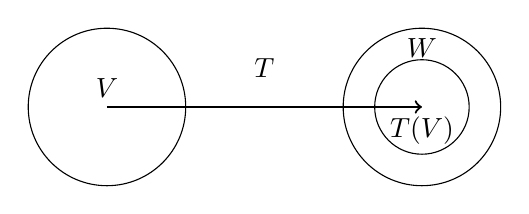
\begin{tikzpicture}
    \draw (1,0) ellipse (1cm and 1cm) node[above] {$V$};
    \draw (5,0) ellipse (1cm and 1cm);
    \draw (5,0.75) node {$W$};
    \draw (3,0.5) node {$T$};
    \draw[thick,->] (1,0) -- (5,0);
    \draw (5,0) ellipse (0.6 cm and 0.6cm) node[below] {$T(V)$};
    
    \end{tikzpicture}
\end{center}
\end{defn}

\end{document}